% !TEX root = ../YourName-Dissertation.tex

\chapter{Precise Analysis on Multiple-trace Attacks}\label{chapter5}
\section{Introduction}
Side-channel attacks allow attackers to infer sensitive information based on the non-functional behaviors of the computer system. Examples of these non-functional behaviors include acoustics, CPU usages, timing, EM signals, etc~\cite{agrawal2002side,hund2013practical,halevi2015keyboard,batina2019csi}. In summary, if the program has different execution behaviors when it processes various keys, an attacker can infer nontrivial information by observing those secret-dependent behaviors. While separate side-channel attacks may have different forms and patterns, we find that a large portion of them share the same fundamental reasons. That is, the memory access pattern is dependent on the original sensitive input.

While removing those dependent memory-access patterns in existing software completely is hard and tedious, fixing some of the most dangerous leakages appears to be a feasible solution. Previous studies on side-channel detections have shown their effectiveness in finding such code patterns. Developers can run the tool to analyze the side-channels leakages and fix those patterns. However, fixing all those leakages seem impossible for the following reasons. First, side-channels are inevitable. For example, tremendous efforts have been made to remove the side-channel vulnerabilities in cryptography libraries in the past decade. However, we still find that there are plenty of side-channel leakages in the latest version of OpenSSL. Second, many side-channel vulnerable versions usually have better performance, such as the T-table lookups in AES, CRT optimizations in RSA, and Fast Discrete Fourier Transform (FDFT) in many media processing libraries. Third, some developers are not interested in fixing side-channels vulnerabilities unless people can show them an attack demo, even for the cryptography developers. For many non-cryptography developers, side-channels are not in the threat model. However, recent studies have shown a series of attacks on the non-cryptography libraries.

The key to solving the problem is looking for a proper metric to assess the side-channel leakages' sensitive level. Many side-channel analysis tools focus on detecting leakages, which is fine because most side-channel attacks target cryptography libraries. For cryptography libraries, even a minor leakage can be severe because the leakage can reduce the encryption algorithm's strength. However, many attacks also exploit non-cryptography libraries and applications like machine learning applications~\cite{yan2020cache,hong2018security}, graphic libraries~\cite{wang2019unveiling}, spell checking tools~\cite{xu2015controlled}, etc. Unlike side-channel attacks on cryptography libraries that exploit one vulnerability at a time, attacks on non-cryptography rely on multiple side-channel leakage sites to retrieve more information. Suppose one program has two leakage sites. It is hard to estimate the total effect of those two leakages. Any two leakages have some underlying complex relationships. That is, the two leakages could be completely independent, which means they leak different information. Alternatively, the two leakages could leak the same information. A typical situation, that is, the two leakage sites, can leak some common knowledge. Apart from that, they have their unique leakages. However, no existing tools that can estimate the total effect of multiple leakage sites. For real-world applications with thousands of lines, it is hard to estimate the amount of leaked information. Attackers can guess the values of some temporary values. But those temporary values contain some knowledge of the original secret buffer.

Second, many side-channel leakage detection tools rely on some techniques like symbolic executions, taint analysis, and abstract interpretations~\cite{203878,182946,Brotzman19Casym,236338}. It is hard to implement those techniques from scratch. So they build the tool on top of existing binary analysis frameworks. Due to the limitations of existing binary analysis frameworks, it is hard to apply existing methods to analyze side-channels in non-cryptography libraries. For many other applications like machine learning, media, and graphic libraries built on the top architecture-dependent libraries (e.g., Intel MKL~\cite{wang2014intel}), those tools can not handle it. Moreover, some binary analysis frameworks (e.g., Angr~\cite{shoshitaishvili2016state}) are limited in analyzing floating-point instructions. But the functionality of those applications heavily depends on floating-point calculations.

Third, while many existing tools can detect side-channel leakages, few of them can assess how severity level of those vulnerabilities~\cite{203878,182946,Brotzman19Casym,236338,217537,Wichelmann:2018:MFF:3274694.3274741}. There are some tools~\cite{182946,Chattopadhyay:2017:QIL:3127041.3127044} that can quantify the information leakage. Those tools can give an upper bound estimation of each leakage site, which is useful to justify the software is secure if the reported leakage is zero. But those tools can not tell software developers how severe each leakage site would be because of the over-approximation they apply when they estimate the amount of leakage. The best way to estimate each leakage's severe level is to exploit the leakage and recover the information. However, the process itself is very tedious and needs a lot of domain knowledge.

To solve the above problem, we propose a method to estimate the effect of side-channel leakages automatically. We compare the side-channel attack to a communication system and use the channel capacity to quantify the amount of the information flow from the original secret to an attacker's observation. The method also allows us to combine multiple leakages sites to retrieve the information. The attack can be seen as a process that reduces the search space of the original sensitive inputs. We use the side-channel vulnerability to divide the input space. If the patterns can uniquely distinguish the input space, then we think the information is leaked totally. However, in real cases, many of those side-channel leakage patterns are not enough to distinguish each leakage site but can still discern some secret inputs. In those cases, we call those partial leakages leaks.

The method consists of three phases. In the first phase, we fuzz the target program with various inputs and collect the memory access information. In the second phase, we map the memory access information with the source code. With the debug information, we can precisely know the address access information of the source code. In the third phase, we exam the source code. If one function has two memory access patterns, then the function is vulnerable to side-channel attacks. Based on the distribution of memory access patterns under different inputs, we quantify each function's side-channel leakage.

This paper makes the following contributions:

\begin{itemize}

  \item We propose a novel method that automatically detects and analyzes the effect of each side-channel leakage site. Our analysis combines information from both the source code and the runtime execution, which makes the method more effective in finding the leakages. The method can combine multiple leakage sites to retrieve more information as well.

  \item We analyze the amount of information leakage from side-channel vulnerabilities based on the channel capacity. We propose a method that can estimate the lower bound of information leakages. The theory can serve as the foundation of future work on quantifying the information leakage based on the fuzzing.

  \item We implement the above method in a tool called \ctool{} and evaluate the tool with several benchmarks and several real-world applications such as OpenSSL, mbedTLS, TinyDNN, and GTK. The results show that our tool can detect and quantify the side-channel leakages effectively. Moreover, the leakage reports given by the \ctool{} can help developers fix the reported vulnerabilities.
\end{itemize}

\section{Background and Threat Model}
In the section, we give an overview of the background knowledge of information theory and present the threat model of the paper.


\subsection{Channel Capacity}
Let $k$ be one of the possible
value of $K$. The Shannon entropy $H(K)$ is defined as
\begin{equation}\label{chapter5:eq1}
  H(K) = - \sum_{k {\in} K}p(k)\log_2(k)
\end{equation}

Shannon entropy can be used to quantify the initial uncertainty about the sensitive information. It measures the amount of information in a system. For example, an AES encryption program takes a 128-bit key as the input. Suppose each key has the equal opportunity and $p_k = 1/ 2^{128}$, then the encryption system has $128 \, \mathit{bits}$ information according to Shannon entropy.


In the paper, we use the channel capacity to describe the amount of information leakages through a channel. In information theory, the channel capacity is used to quantify the rate of information can be reliably transmitted over a channel. If we use $K$ to represent the input secrets and $O$ to represent the output observation. The channel capacity ($C$) is defined as

\begin{equation}\label{chapter5:eq2}
  C(K;O) = \max_{p(x)} I(K;O)
\end{equation}
Here $I(K;O)$ is the mutual information between $K$ and $O$.
\begin{equation} \label{chapter5:eq3}
  I(K;O) = \sum_{k {\in} K}{\sum_{o {\in} O}{p(k, o)\log_2\frac{p(k, o)}{p(k)p(o)}}}
\end{equation}

While the channel capacity in general situations is hard to compute, we consider two special channels.

\subsubsection{Noiseless Lossless Channel}
An information channel is noiseless and lossless if

\begin{equation} \label{chapter5:eq4}
  C(K;O) = \max_{p(k)} I(K;O) = \max_{p(k)} H|O| =\max_{p(k)} H|K|
\end{equation}
$|K|$ represents the number of symbols in $K$.

Figure~\ref{fig:channel}(a) shows an example of the type of the channel. Under the circumstance, we always have $P(o_i/k_i) = 1$ and $P(k_i/o_i) = 1$. As we can see, the channel have the unique output ($o \in O$) for every input ($k \in K$).

\begin{figure}
  \begin{minipage}{0.45\linewidth}
    \resizebox{\linewidth}{!}{

      \begin{tikzpicture}[ele/.style={fill=black,circle,minimum width=.8pt,inner sep=1pt},every fit/.style={ellipse,draw,inner sep=-2pt}]
        \node[ele,label=left:{\normalsize	 $k_1$}] (a1) at (0,4) {};
        \node[ele,label=left:{\normalsize	 $k_2$}] (a2) at (0,3) {};
        \node[ele,label=left:{\normalsize	 $k_3$}] (a3) at (0,2) {};
        \node[ele,label=left:{\normalsize	 $k_4$}] (a4) at (0,1) {};

        \node[ele,,label=right:{\normalsize	 $o_1$}] (b1) at (4,4) {};
        \node[ele,,label=right:{\normalsize	 $o_2$}] (b2) at (4,3) {};
        \node[ele,,label=right:{\normalsize	 $o_3$}] (b3) at (4,2) {};
        \node[ele,,label=right:{\normalsize	 $o_4$}] (b4) at (4,1) {};

        \node[draw,fit= (a1) (a2) (a3) (a4),minimum width=2cm] {} ;
        \node[draw,fit= (b1) (b2) (b3) (b4),minimum width=2cm] {} ;
        \draw[->,thick,shorten <=2pt,shorten >=2pt] (a1) -- (b1);
        \draw[->,thick,shorten <=2pt,shorten >=2] (a2) -- (b2);
        \draw[->,thick,shorten <=2pt,shorten >=2] (a3) -- (b3);
        \draw[->,thick,shorten <=2pt,shorten >=2] (a4) -- (b4);
      \end{tikzpicture}
    }
    \caption*{(a) Noiseless Lossless}
  \end{minipage}
  \hfill
  \begin{minipage}{0.45\linewidth}
    \resizebox{\linewidth}{!}{

      \begin{tikzpicture}[ele/.style={fill=black,circle,minimum width=.8pt,inner sep=1pt},every fit/.style={ellipse,draw,inner sep=-2pt}]
        \node[ele,label=left:{\normalsize $k_1$}] (a1) at (0,4) {};
        \node[ele,label=left:{\normalsize $k_2$}] (a2) at (0,3) {};
        \node[ele,label=left:{\normalsize $k_3$}] (a3) at (0,2) {};
        \node[ele,label=left:{\normalsize $k_4$}] (a4) at (0,1) {};

        \node[ele,,label=right:{\normalsize $o_1$}] (b1) at (4,4) {};
        \node[ele,,label=right:{\normalsize $o_2$}] (b2) at (4,3) {};
        \node[ele,,label=right:{\normalsize $o_3$}] (b3) at (4,2) {};
        \node[ele,,label=right:{\normalsize $o_4$}] (b4) at (4,1) {};

        \node[draw,fit= (a1) (a2) (a3) (a4),minimum width=2cm] {} ;
        \node[draw,fit= (b1) (b2) (b3) (b4),minimum width=2cm] {} ;
        \draw[->,thick,shorten <=2pt,shorten >=2pt] (a1) -- (b1);
        \draw[->,thick,shorten <=2pt,shorten >=2] (a2) -- (b2);
        \draw[->,thick,shorten <=2pt,shorten >=2] (a3) -- (b2);
        \draw[->,thick,shorten <=2pt,shorten >=2] (a4) -- (b2);
      \end{tikzpicture}
    }
    \caption*{(b) Noiseless Loss}
  \end{minipage}
  \caption{Two Kinds of Channels}\label{fig:channel}
\end{figure}


\subsubsection{Noiseless Loss Channel}
In reality, noiseless loss channel is more common. We define the channel is noiseless loss if

\begin{equation} \label{chapter:eq:5}
  C(K;O) = \max_{p(x)} I(K;O) = \max_{p(x)} H |O| = \log_2 {|O|}
\end{equation}

Figure~\ref{fig:channel}(b) shows the example of the type of the channel. Once the input symbol is determined, the output symbol is also determined. As we can see, the channel has a unique output ($o \in O$) for every input ($k \in K$).


\subsection{Threat Model and Notation}


We consider an attacker who shares the same hardware resource with the victim. The attacker may not know the memory access the victim program accesses directly. Still, he can infer whether some memory addresses are accessed or not at various granularities after \textit{each run} of the victim program. We call the memory access information as the observation ($O$) in the rest of the paper. This is a typical scenario for most side-channel attacks.  We also assume the attacker can have access to the source code of the victim program ($\beta$). It is a valid assumption since most side-channel attacks target open-source software. Also, like recent works, we assume the attacker has a noise-free observation. For some side-channel channels like the controlled-channel attacks, it is already true. The program ($\beta$) has $K$ as the sensitive input. $K$ is a finite set that consists of every possible key ($k \in K$). The program also takes known messages $M$ as the input.

\begin{figure}[ht]
  \centering
  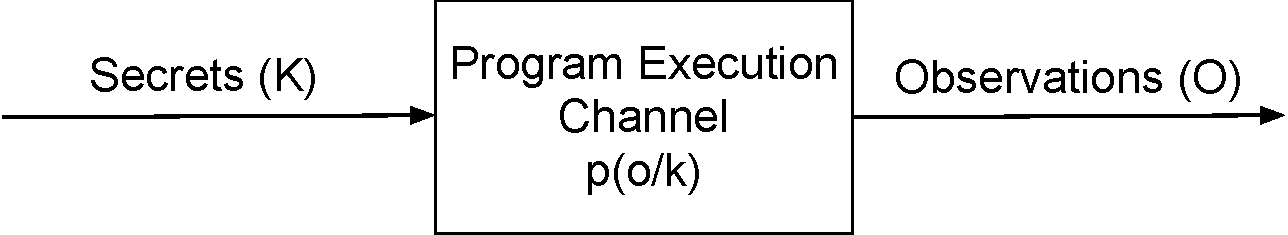
\includegraphics[width=.8\columnwidth]{./figures/chapter5/channel.pdf}
  \caption{The relationship between the side-channel attack and the channel capacity. For a deterministic program, the side-channel attack can be seen as the communication between the observation ($o \in O$) and the secret ($k \in K$) via a discrete memoryless channel.}
  \label{fig:side_channel}
\end{figure}

With the above definitions, we define the following mapping between $\beta$,
$K$, $M$, and $O$:

\begin{displaymath}
  \beta(K, M) \rightarrow O
\end{displaymath}


Side-channel attacks can be seen as a process that infers the secret ($K$) based on the observations ($O$) shown in the figure~\ref{fig:side_channel}. As an attacker, he can observe the memory address of the victim program. He wants to infer the original secret ($k$) based on the observation. We also assume the attacker knows the known message $m \in M$. In the rest of paper, we use $\beta(K) \rightarrow O$ to denote a victim program with side-channel vulnerabilities.


In this paper, we consider three types of granularity: byte (1 Byte), cache line size (64 Bytes), page size (4 KBs). To the best of our knowledge, the three types of granularities can cover most of the side-channel attacks in literature.

\section{Method}
In this section, we first provide two examples that show how we rank the side-channel vulnerability. After that, we prove that our method is the conservative estimate of the amount of each leakage.

\subsection{An Example}
Figure~\ref{fig:example1} shows a function that is vulnerable to side-channel attacks. The function takes an input secret from the caller. Depending on the value of the secret, it may access different values at line 7. Suppose an attacker can observe which item in the table \textsf{T} is accessed. He can infer the secret based on the observation.

\begin{figure}[h]
  \begin{minipage}{0.6\linewidth}
    \begin{lstlisting}[xleftmargin=.15\textwidth,xrightmargin=.30\textwidth]
void bar(uint8_t secret)
{
  uint8_t T[128];
  uint8_t index = 0, t;
  int i;
  index = (index+secret)%128;
  t = T[index];
  ...
}
\end{lstlisting}
  \end{minipage}
  \hfill
  \begin{minipage}{0.4\linewidth}
    \resizebox{0.8\textwidth}{!}{%

      \begin{tabular}{cccccccccc}
        \toprule
        \diagbox{S}{T} & 0 & 1 & 2 & 3 & 4 & 5 & 6 & 7 & ... \\
        \midrule
        0              & A &   &   &   &   &                 \\
        1              &   & A &   &   &   &                 \\
        2              &   &   & A &   &   &                 \\
        3              &   &   &   & A &   &                 \\
        4              &   &   &   &   & A &                 \\
        5              &   &   &   &   &   & A &             \\
        6              &   &   &   &   &   &   & A           \\
        7              &   &   &   &   &   &   &   & A       \\
        \bottomrule
      \end{tabular}%
    }
  \end{minipage}
  \caption{A severe leakage.}\label{chapter5:fig:example1}
\end{figure}

To assess the sensitive level of the vulnerability, we use the sampling method to estimate the leakage. Suppose we give the function input from $0, 1, \dots, 7$ and observe the array $T$, we can find each different input has one unique observation. Therefore, the secret can be uniquely determined.

\begin{figure}[h]
  \begin{minipage}{0.60\linewidth}
    \begin{lstlisting}[xleftmargin=.15\textwidth,xrightmargin=.30\textwidth]
void bar(uint8_t secret)
{
  uint8_t T[128];
  uint8_t index = 0, t;
  int i;
  index = (index+secret)%128;
  t = T[index % 4];
  ...
}
\end{lstlisting}
  \end{minipage}
  \hfill
  \begin{minipage}{0.4\linewidth}
    \resizebox{0.8\textwidth}{!}{%

      \begin{tabular}{cccccccccc}
        \toprule
        \diagbox{S}{T} & 0 & 1 & 2 & 3 & 4 & 5 & 6 & 7 & ... \\
        \midrule
        0              & A &   &   &   &   &                 \\
        1              &   & A &   &   &   &                 \\
        2              &   &   & A &   &   &                 \\
        3              &   &   &   & A &   &                 \\
        4              & A &   &   &   &   &                 \\
        5              &   & A &   &   &   &   &             \\
        6              &   &   & A &   &   &   &             \\
        7              &   &   &   & A &   &   &   &         \\
        \bottomrule
      \end{tabular}%
    }
  \end{minipage}
  \caption{A minor leakage. }\label{chapter5:fig:example2}
\end{figure}
On the other hand, the second example also has side-channel leakages at line 7. However, the leakage is slightly different. Still, we test the program with input from $0, 1, \dots, 7$. However, we find the attacker can not uniquely determine the secret based on the observation of table $T$, for example. Both $0$ and $4$ read the first item of the table. Therefore, we think the vulnerability is minor than the previous one. Here comes the definition of the amount of leaked information of the vulnerability.


\begin{mydef}
  \label{chapter5:def}
  Suppose we have a program $\beta$ with the input set $K$. We randomly select $k_1, k_2, \dots, k_n \in K' \subseteq K$ as the input. We denote it as
  $$\beta(K') \rightarrow	O'$$

  Here $O$ is a set that consists of various observations $o_1, o_2, \dots, o_m$. The amount of leaked information $L_{\beta(K')\rightarrow O'}$ based on the observation ($o$) is
  $$L_{\beta(K')\rightarrow O'} = H(O') $$
\end{mydef}


With Definition~\ref{chapter5:def}, we can calculate the information leakage in Figure~\ref{chapter5:fig:example1} and Figure~\ref{chapter5:fig:example2} respectively. In Figure~\ref{chapter5:fig:example1}, we have $8$ kinds of observations and each observation is uniformly distributed. Therefore, the information leakage is $log_2{8} = 3$ bits. In Figure~\ref{chapter5:fig:example2}, we have $4$ kinds of observations and each observation is also uniformly distributed. Therefore, the information leakage is $log_2{4} = 2$ bits. We test the program with $8$ inputs. Therefore, the Shannon entropy of the original K $H(K)$ is also $3\,\mathrm{bits}$. According to Equation~\ref{chapter5:eq1}. the secret-dependent data accesses in Figure~\ref{chapter5:fig:example1} can leak the sensitive information totally.

\subsection{A Conservative Estimation}
In this section, we prove Definition~\ref{chapter5:def} is the conservative estimation of the amount of leaked information based on the channel capacity.

\begin{theorem}\label{the1}
  If an attacker launches a side-channel attack on deterministic programs, then the channel between the secret and the observation is a noiseless loss channel.
\end{theorem}

\begin{myprof}
  According to information theory,
  \begin{align*}
    I(K;O) & = H(O) - H(O|K)                                \\
           & = H(O) - \sum_{k {\in} K }{p(o|k)\log_2p(o|k)}
  \end{align*}
  For a deterministic program, $p(o|k)=1$. As a result, $H(O|K) = 0$.
  \begin{align*}
    C(K;O) = \max_{p(k)} I(K;O) = \max_{p(k)} H |O|
  \end{align*}
\end{myprof}

With THEOREM~\ref{the1}, we can have
\begin{align*}
  \max_{p(k)} H |O| >= \max_{p(k')} H |O'| >= H |O'|
\end{align*}

Accordingly, if Definition~\ref{chapter5:def} says the vulnerability leakage has $m$ bits of leakages, then the vulnerability can have at least $m$ bits of leakages. We can use the definition to detect those severe leakages. In the examples of Figure~\ref{chapter5:fig:example1} and Figure~\ref{chapter5:fig:example2}, because the secret input range from $0$ to $255$, we can calculate the precise value of the amount of information leakage by iterating each input keys. In Figure~\ref{chapter5:fig:example1}, each item in the array could be read. Therefore, the channel capacity in Figure~\ref{chapter5:fig:example1} is $\log_2{128} = \,7\, \mathrm{bits}$. In Figure~\ref{chapter5:fig:example2}, there could be $4$ kinds of information, so the information leakages defined by channel capacity is $\log_2{4} = \,2\, \mathrm{bits}$. Compared with the result from Definition~\ref{chapter5:def}, we can see that the amount of leakages by Definition~\ref{chapter5:def} is a conservative estimation.

\section{Align Address Access Across Multiple Executions}
We compare address accesses of different executions generated by different inputs to quantify the amount of leakage information. A meaningful comparison requires that we align executions across multiple runs before we quantify the leakage. In this work, we combine the information from both the source code and the binary executable to align the memory access during the execution.


\begin{figure}[h]
  \begin{minipage}{0.45\linewidth}
    \begin{lstlisting}[numbers=none,xleftmargin=.1\textwidth,xrightmargin=.2\textwidth]
uint8_t *T = malloc(4);
if (T==NULL) exit(1);
...
t = T[i];    
\end{lstlisting}
  \end{minipage}
  \hfill
  \begin{minipage}{0.5\linewidth}
    \resizebox{\textwidth}{!}{

      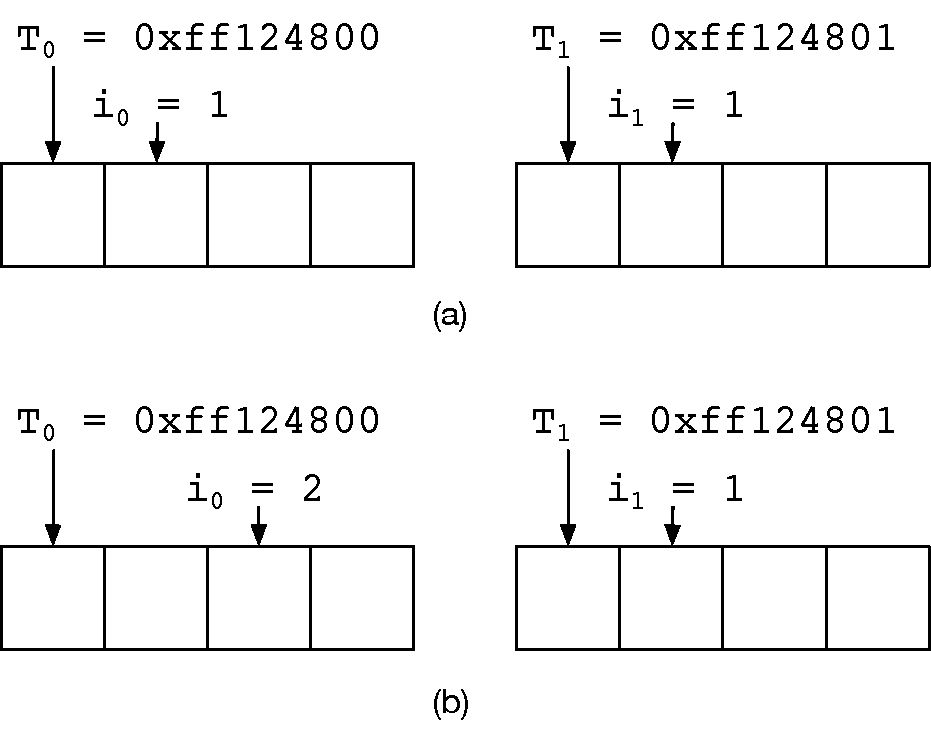
\includegraphics[width=\columnwidth]{./figures/chapter5/align.pdf}

    }
  \end{minipage}
  \caption{Without proper address alignment, there could be many false positives and false negatives.}\label{fig:align}
\end{figure}

Considering the example in figure~\ref{fig:align}, it read the data from the array \textsf{T} based on the index (i). If index (i) is associated with a key, it could be a side-channel vulnerability. Unlike the example in the previous section, the array \textsf{T} is on the heap. Data on the heap are allocated in different addresses each time. Suppose during the first run, \textsf{T} is allocated at the address \textsf{0xff124800} and \textsf{T} is allocated at the address \textsf{0xff124801} at the second run. For the example in Figure~\ref{fig:align}(a), the index that is used to access the array is always $1$, so it should not be a side-channel vulnerability here, however, because the based address is different. So we get two different memory accesses. Under the circumstance, it is a false positive. Besides, it can cause false negatives, as the example shown in Figure~\ref{fig:align}(b). In the example, different keys lead to different indexes. However, as $T_0 + i_0$ equals to $T_1 + i_0$, \ctool{} can not observe the difference here, which can cause a false positive.

\textbf{Our Strategy: } We assign a value for each memory location~\cite{sumner2010memory}. The value should satisfy the following characteristics.
\begin{itemize}
  \item \textbf{Uniqueness.} At any point during the execution, different memory cells must have a different value.
  \item \textbf{Alignment.} The same memory cell across multiple executions should share the same value.
\end{itemize}

There are some possible solutions that can assign the value.
\textbf{Run-time Information.} One example here is the concrete memory address during the runtime. Such a value satisfies the uniqueness characteristic. However, as the example shown in Figure~\ref{fig:align}, it does not have the alignment property.
\textbf{Source Code Information.} Alternatively, we can use the information from the source code. Recent work~\cite{sumner2010memory} proposes using the execution point that allocates the memory cell as the index and tracking the pointer arithmetic to track the pointer that points to the memory. However, such a method may miss the alias symbol that points to the same memory cell.

We propose to combine both the information from the source code and the runtime to align the memory access during the execution. At the point the memory is allocated, we use the tuple $(start\ address, length)$ to represent the buffer. In the following execution, we check if any memory access falls into the range of those tuples. If so, we add the memory access into the tuple. After the execution, the tuple can be mapped into the location of the source code, and we only compare the memory access that belongs to the same lines in the source code.

\section{Multiple Leakages Sites}
Real-world software can have many side-channel vulnerabilities. Those vulnerabilities may spread throughout the whole program. An adversary may exploit more than one side-channel vulnerabilities to gain more information~\cite{7163052, 191010}. In order to precisely quantify the
total information leakage, we need to know the relation of those leakage sites. 

\begin{figure}[h]
\begin{minipage}{0.4\linewidth}
\begin{lstlisting}
void function1(uint8_t* secret)
{
  uint8_t k1, k2;
  k1 = secret[1];
  k2 = secret[2];
  if (k1 > k2)
    a();
  if (k1 + k2 < 256)
    b();
  ...
}
\end{lstlisting}\caption*{(a) Independent Leakages}
\end{minipage}
\hfill
\begin{minipage}{0.4\linewidth}
\begin{lstlisting}
void function2(uint8_t* secret)
{
  uint8_t k1, k2;
  k1 = secret[1];
  k2 = secret[2];
  if (k1 + k2 > 128)
    c();
  if (k1 > 32)
    d();
  ...
}
\end{lstlisting} \caption*{(b) Dependent Leakages}
\end{minipage}
\caption{Multiple leakage sites. The two leakage sites in Figure (a) leak different information. But the leaked information in Figure (b) has some overlaps. }\label{chapter5:fig:multiple}
\end{figure}

Considering the examples in Figure~\ref{chapter5:fig:multiple}, Figure~\ref{chapter5:fig:multiple}(a) show a code snippet with two leakage sites at line 6 and line 8 respectively. For example, if an adversary observes that function \textsf{a} executes, then the attacker can infer the first byte in buffer \textsf{secret} is larger than the second byte.  Similarly, if an adversary observes that function \textsf{b} executes, then the attacker can infer that the sum of the first two bytes in buffer \textsf{secret} is smaller than $256$. The interesting part here is that if the attacker observes that function \textsf{a} executes, then he still has zero knowledge about the function \textsf{b}. The two leakage sites in Figure~\ref{chapter5:fig:multiple}(b) are different. If an attacker observes function \textsf{c} executes, then it is likely the attacker can observe that function \textsf{d} also executes. 

Suppose one program has two side-channel vulnerabilities A and B, which can leak $L_A$ and $L_B$ bits respectively, according to the definition~\ref{chapter5:def}. 
Depending on the relation between A and B, the total leaked information $L_{\mathit{total}}$ will be:

\subsection{Independent Leakages}
If A and B are independent leakages, the total information leakage will be:
\[L_{\mathit{total}} = L_A + L_B \]

\subsection{Dependent Leakages}
If A and B are dependent leakages, the total information leakage will be:
\[\max{\{L_A, L_B\}}  \leq L_{\mathit{total}} < L_A + L_B\]

We use the chi-square test to check if two leakage sites are independent. A chi-squared test can determine if there is a relationship between two categorical variables. Suppose we can summarize the data in a $r*c$  two-way contingency table. The chi-square test statistic and the degrees of freedom $v$ are calculated with the below formula:
\[\tilde{\chi}^2=\sum_{k=1}^{rc} \frac{(O_k - E_k)^2}{E_k} \qquad	 v = (r - 1)(c - 1)\]
Here $O$ is the observed value, and $E$ is the expected value. A low value means that there is a high correlation between the two variables. 

The null hypothesis is that the two leakages are independent.
We generate random inputs as the secret and record the memory access for each execution. For each time, the execution is independent of the previous execution. The times of the same observation for each event should satisfy the normal distribution. After that, we can use the chi-squared test to test whether the two leakage sites are independent.

\begin{figure}[h]
  \begin{minipage}{0.40\linewidth}
      \begin{tabular}{rrrr}
        \toprule
        & $a$ & $\lnot a$  & total\\
        \midrule
        $b$   & 255 (255.5) & 253 (252.5) &   508  \\
        $\lnot b$   & 260 (259.5)  & 256 (256.5) &    516   \\
        total &   515 &  509   & 1,024   \\
        \bottomrule
      \end{tabular}\caption*{(a)}
  \end{minipage}
\hspace{-15pt}
\hfill
\hspace{-15pt}
  \begin{minipage}{0.40\linewidth}
      \begin{tabular}{rrrr}
        \toprule
        & $c$ & $\lnot c$  & total\\
        \midrule
        $d$   & 809 (764.8) & 82 (126.2) & 891    \\
        $\lnot d$   & 70 (114.2)  & 63 (18.8)&  133     \\
        total &  879 &  145  & 1,024    \\
        \bottomrule
      \end{tabular}\caption*{(b)}
  \end{minipage}
  \caption{The contingency table for the experiments. The numbers in the bracket are expected values. }\label{chapter5:fig:con_table}
\end{figure}


Assume we generate $1024$ random inputs and record the memory access each time. For the example in Figure~\ref{chapter5:fig:multiple}, we use $a$ to denote the function \textsf{a} executes and $\lnot a$ to denote the function \textsf{a} does not execute during the execution. After calculating the number of the same observation, we get the contingency table shown in Figure~\ref{chapter5:fig:con_table}. Suppose the observations of function \textsf{a} and function \textsf{b} are independent. We calculate the expected value for the observation $ab$ based on the frequency.
\[ E_{ab} = \frac{(255+256)*(255+253)}{1024} = 255.5\]
Similarly, we calculate the rest expected values with the hypothesis that the leakages are independent and fill in them in Figure~\ref{chapter5:fig:con_table}. The degree of freedom $v$ is $(2-1)*(2-1) = 1$.

Based on the equation, we calculate the chi-square test statistic for two leakage sites in Figure~\ref{chapter5:fig:multiple} (a) and (b).

\[\tilde{\chi}^2_{a}= \frac{(255.5-255)^2}{255.5} + \frac{(252.5-253)^2}{252.5} + \frac{(259.5-260)^2}{259.5} + \frac{(256.5-256)^2}{256.5} = 0.004\] 
\[\tilde{\chi}^2_{b}= \frac{(764.8-809)^2}{764.8} + \frac{(126.2-82)^2}{126.2} + \frac{(114.2-70)^2}{114.2} + \frac{(18.8-63)^2}{18.8} = 139.1\] 

According to Chi-squared distribution table, we have the probability $p\approx0.95$ to accept the null hypothesis for the two leakages in Figure~\ref{chapter5:fig:multiple} (a). We have the probability $p\approx0.00$ to accept the null hypothesis for the two leakages in Figure~\ref{chapter5:fig:multiple} (b). Therefore, we infer that the two leakages in Figure~\ref{chapter5:fig:multiple} (a) are independent. And the two leakages Figure~\ref{chapter5:fig:multiple} (b) are dependent. In this paper, for any two leakages, if $p < 0.03$, we think the two leakage sites are independent. We use the above method to test if any two leakage sites are independent for each leakage point. We combine them into a leakage are calculate the total amount of the leakage.
\section{Design}
In this section, we explain the implementation of \ctool{}.
We first present the overview of \ctool{}. After that, we discuss some design details to implement \ctool{}.

\subsection{Overview}
Figure~\ref{chapter5:fig:workflow} shows an overview of our side-channel leakages quantification tool. Given the source code of the victim program, \ctool{} can find the address-based side-channel leakages by fuzzing the victim program. To assist the illustration, we divide the workflow of ~\ctool{} into three steps. For the first step, we build the target program from the source code. After that, we give them random inputs to the victim program and run the target program and record each of the addresses in the binary file is hit or not, and store the information in a bitmap. Next, we analyze the side-channel leakage from the address access bitmap. We split the address space into several segments to speed up the comparison according to Meta information. Finally, \ctool{} Generate the final leakage report. For each leakage site, \ctool{} gives the conservative estimation of the information leakage. Every leakage site in the report is a true leakage, and there are no false positives.

\begin{figure}[ht]
  \centering
  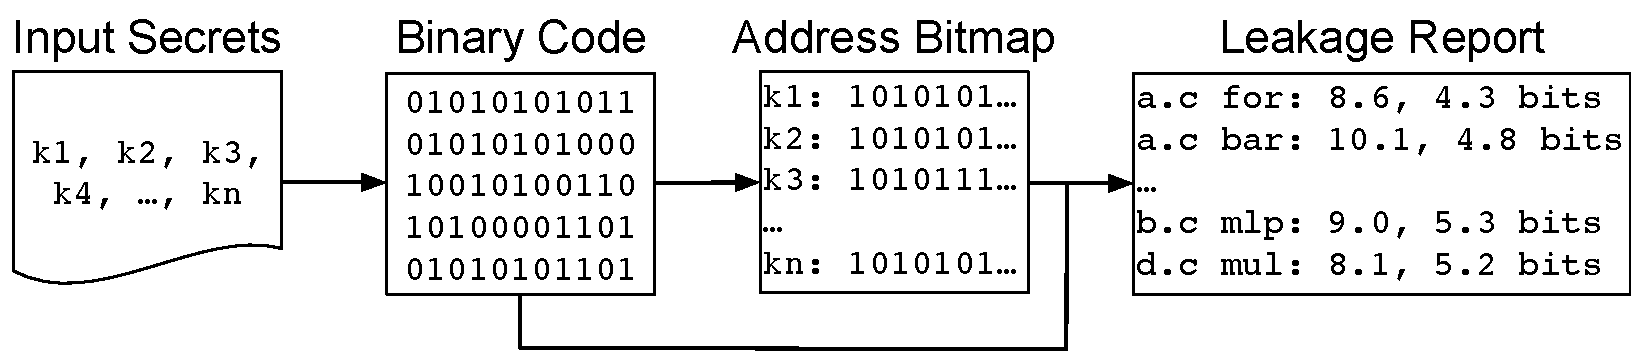
\includegraphics[width=\columnwidth]{./figures/chapter5/workflow.pdf}
  \caption{The workflow of \ctool{}. We try to divide the \ctool{} into three steps to assist the illustration. }\label{chapter5:fig:workflow}
\end{figure}

\subsection{Step 1: Fuzzing}
After we build the software into the binary executable, we give the binary code the random inputs. For cryptography libraries, the input is the encryption key. For non-cryptography libraries, the input could be images, text, and information in other formats. Encryption algorithms like AES, DES take an array representing the secrets. We generate the random input by flipping each bit of the keys. Some other programs also take a buffer as the input. The buffer may contain the redundancy information and follow a specific format. So not any input that satisfies the input length is a valid input. Under the circumstance, we have a dictionary that contains the input. For example, Crypto libraries usually take PKCS \#1 as the input of RSA private key. We use some other tools to generate a list of valid keys and use the key to sample the program. Due to the enormous search space, we can not iterate every input. However, our method can give a conservative estimate of each leakage site.
\subsection{Step 2: Address Record}
Next, we record the memory access information based on the input secret. We use the dynamic binary instrumentation (DBI) tool to record whether a particular memory access information is accessed or not. Inspired by the AFL and Valgrind, we use the bitmap to represent whether a particular memory is accessed or not. For example, the bitmap ${0101}$ of address $address_1, address_2, address_3, address_4$ means that $address_2, address_4$ are hit during the execution. During the execution, the direct information we get is the virtual memory address (VMA). However, we transfer the address into the offset (Load Memory Address (LMA)) in the original binary file. It has two benefits. First, modern computer systems employ the Address Space Layout Randomization (ASLR). With ASLR, the operating system randomly puts the enclave code and data at various memory offset. As a result, the code will get different execution traces even for the same input because the enclave image is loaded at a different address each time. Second, it helps us find the leakage site in the source code.

We rely on the program header and symbol information to recover the offset in the binary. During the loading process, the operating system maps each segment into a contiguous memory region. So the offset of the virtual memory address between the code within the same segment is the same as the offset within the binary file. We choose the start address of some common functions (e.g, $main$) ($b$) as the navigation function. We get the virtual memory address of the start of the function ($\mathit{VMA_b}$) from the DBI tool and the load memory address of the function ($\mathit{LMA_b}$) from the symbol information. For any virtual address, we use Equation~\ref{equ:eq6} to calculate the offset in the original address.
\begin{equation}\label{equ:eq6}
  \mathit{LMA_a} = \mathit{LMA_b} - VMA_b - VMA_a
\end{equation}

There are two kinds of memory accesses: accesses to the code and accesses to the data.
\begin{itemize}
  \item Code Access. The memory address of the code is the value of $rip$ register. However, the length of x86 instructions can be from 1 byte to 15 bytes. For instructions whose length is longer than one byte, we also update the address after the value $rip$ until the address reaches the instruction's boundary.
  \item Data Access. For instructions with memory access, we identify all the operands of each instruction and. Same as the code address, the instruction can read or write multiple bytes one time.  Instructions like \textsf{push} and \textsf{pop} have implicit memory access. We all update the bitmap of the address correspondingly.
\end{itemize}

\subsection{Step 3: Leakages Detection and Quantification}
In this step, we detect and quantify the side-channel leakage. For each $k \in K$, we have a boolean number ($0$ or $1$) to describe whether the address $addr$ is accessed or not during the execution when the input is $k$. For the brevity of description, For the brevity of description, we use $B^{addr}_{k_i}$ to denote the boolean number.



\subsubsection{Various Granularities Side-channel Detection}
\ctool{} can detect the side-channel vulnerabilities in different granularities. For each granularity, we calculate a new bitmap that represents access information of each unit. We have the bitmap of the memory access at the byte level. An attacker who has the coarse-grained observation at address space may not distinguish the address difference. For example, modern X64 computer systems use 48-bit virtual memory addresses. The top 36 bit of the virtual address is called Virtual Page Number (VPN), and the bottom 12 bits of the virtual address is called offset. The memory management unit (MMU) transfers the virtual address into the physical address by mapping the Virtual Page Number (VPN) into the Physical Page Number (PPN) while keeping the offset of the address. So two addresses with the Same VPN but different offset are not distinguishable by an attacker who only has the page-level observation.

Suppose a program reads one byte at memory $\mathsf{0x7ffff7ffd001}$ when the secret is $k_1$ and reads a different byte at memory $\mathsf{0x7ffff7ffda01}$ when the secret is $k_2$, an attacker who has the page-level observation can not launch the attack but an attacker who launches the cache attack can know the input is $k_1$ or $k_2$. We update the new bitmap of the large unit by merging the bitmaps of small units that fall into the large unit. That is, $\forall addr_1, addr_2, \dots, addr_n \in addr_N, B^{addr_N}_{k_i} = B^{addr_1}_{k_i} \lor,\dots,\lor B^{addr_N}_{k_n}$.


\subsubsection{Leakage Detection} The access of the address is secret-dependent if $ \exists\, k_{i1}, k_{i2} \in K, \, B^{addr}_{k_i1} \oplus  B^{addr}_{k_i2} =1 $. In the paper, we perform the logical exclusive OR operation on every boolearn value in the same address. If the result is $1$, then the address is vulnerable to the side-channel attacks.

\begin{myexample}
Suppose we sample a program from $k1$ to $k8$ and record the memory access at the granularity of each byte from $\mathsf{7ffff7ffd000}$ to $\mathsf{7ffff7ffd03f}$ (One cache line). We perform the bit-wise or operation of each address with the address range. Because the cache line is always accessed. We think it is not a leak here.
\begin{center}
  \begin{tabular}{c}
    {
      \begin{lstlisting}[frame=none]
              k1  k2  k3  k4  k5  k6  k7  k8   Result  
7ffff7ffd000   1   0   1   0   1   1   0   1 
7ffff7ffd000   0   1   1   0   1   1   1   1 
7ffff7ffd000   1   1   1   1   1   1   0   1 
7ffff7ffd000   1   0   1   0   1   1   1   1 
...
7ffff7ffd03f   1   0   1   0   1   1   1   0  
cache line     1   1   1   1   1   1   1   1    0 (No Leaks)
\end{lstlisting}
    }
  \end{tabular}
\end{center}
\end{myexample}

\subsubsection{Estimate The Leaked Information}
According to Definition~\ref{chapter5:def}, we quantify the information leakage based on the distribution of the observation. If we calculate the information leakage from a $4MB$ memory area, then the length of the byte-level bitmap is $4*1024*1024 = 4194304$. While it is possible to compute the distribution of the bitmap theoretically, it is hard to compare the bitmap of such length in practice.

To solve the problem, we use the debug information to split the bitmap into several segments and map the leakage site into the source code location. Each segment maps the address access situation of the function in the source code. In our setting, the max length of the bitmap of each segment is $1024$, the length of \textsf{uint1024\_t}. So we can put the bitmap into a variable. The split operation eases the computation. However, it also adds the limitation of the max address range when we quantify the side-channel leakage shown in Table~\ref{tab:size_limitation}. We think the range of the memory is big enough for us to quantify most of the cache side-channel attacks.

\begin{table}[h]
  \centering
  \resizebox{0.8\textwidth}{!}{%

    \begin{tabular}{llll}
      \toprule
      Granularity & Byte       & Cache Line (64 Bytes) & Memory Page (4 KB) \\
      \midrule
      Range       & 1024 Bytes & 64 KB                 & 4 KB               \\
      \bottomrule
    \end{tabular}
  }
  \caption{The maximum range address range when we quantify the amount of the leakage with different granularity.}
  \label{tab:size_limitation}
\end{table}

After that, we traverse the bitmap for each $k$ and count it to get the distribution of the bitmap. The counting process is like traversing a binary tree.

\begin{myexample}
Shown in Figure~\ref{fig:design:example2}, we have the following observation from $k_1$ to $k_8$, then we count the distribution of  the observation. The process is like traversing a binary tree and increase the counter of the child node. According to Definition~\ref{chapter5:def}, the amount of the leakage is $1.4$ $\mathit{bits}$.

\begin{displaymath}
  H(O') = - \frac{3}{8}*\log_2{\frac{3}{8}}- \frac{1}{2}*\log_2{\frac{1}{2}}
  - \frac{1}{8}*\log_2{\frac{1}{8}} = 1.4 \,\mathrm{bits}
\end{displaymath}

\begin{figure}[h]
  \begin{minipage}{0.3\linewidth}
    \resizebox{\linewidth}{!}{
      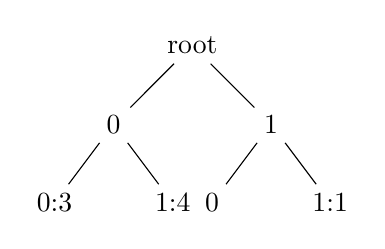
\begin{tikzpicture}
        [level distance=1cm,
          level 1/.style={sibling distance=2cm},
          level 2/.style={sibling distance=1.5cm}]
        \node {root}
        child {node {0}
            child {node {0:3}}
            child {node {1:4}}
          }
        child {node {1}
            child {node {0}}
            child {node {1:1}}
          };
      \end{tikzpicture}

    }\end{minipage}
  \hfill
  \begin{minipage}{0.2\linewidth}
    {
      \begin{lstlisting}[frame=none, numbers=none]
k1  00
k2  01
k3  01
k4  01
k5  00
k6  01
k7  11
k8  00
\end{lstlisting}
    }
  \end{minipage}
  \hfill
  \begin{minipage}{0.25\linewidth}
    \resizebox{\linewidth}{!}{

      \begin{tabular}{ll}
        \toprule
        Observation & P     \\
        \midrule
        00          & $3/8$ \\
        01          & $1/2$ \\
        10          & 0     \\
        11          & $1/8$ \\
        \bottomrule
      \end{tabular}
    }
  \end{minipage}
  \caption{Example 2}\label{fig:design:example2}
\end{figure}
\end{myexample}


\section{Implementation}
We have implemented a prototype of \ctool{}. It takes an input of ELF binary as well as the source code of the corresponding problem. The front-end of \ctool{} is implemented in Python. It can generate random inputs and test the program with those inputs many times.  The address record part is implemented as an Intel Pin tool plugin in C++ to record the bitmap for each input. The main component uses \textsf{libelfin}, an open-source library to parse ELF binaries and read DWARF debug information. The current implementation can support  64-bits ELF binary in Linux. 

\section{Evaluation}
In this section, we evaluate \ctool{} on real-world software trying to answer the following questions:

\begin{itemize}
\item \textbf{Effectiveness:} Can \ctool{} quantify the information leakage with an conservative estimation? If so, what is the loss compared with the real leakage?
\item \textbf{Performance:} What are overhead costs of \ctool{}?
\item \textbf{Usage:}  Can \ctool{} help developers find and fix side-channel leakages?
\end{itemize}

\textbf{Evaluation setup.} We run all the following experiments in a machine with Ubuntu 18.04 LTS. The machine equips with a 2.30GHz Intel Core i9-9880 CPU with 16GB RAM memory. We use the default release settings to build the software's source code into ELF 64-bit executables with GCC 7.5. 

\textbf{Benchmarks.} 
We collect benchmarks from real-world applications and libraries. Our test programs cover applications from diverse functionalities, including small programs, cryptography, machine learning applications, and graphic libraries. 



\textit{Cryptography Applications:} Our benchmarks include the most popular cryptography libraries, such as mebdTLS, OpenSSL, Libgcrypt, and wolfSSL. Encryption ciphers can be divided into three categories:  symmetric ciphers and asymmetric ciphers. For stream ciphers, we use RC4. For symmetric ciphers, we choose AES. We also evaluate the tool on RSA, a widely used algorithm in the public-key cryptosystem.

\textit{Machine Learning Applications:} We evaluate the tool on TinyDNN, a dependency-free deep learning framework in C++.

\textit{Graphic Libraries:} We evaluate the tool on GTK, a popular graphic library. Previous research has demonstrated attacks to infer the keystroke.

\begin{sidewaystable}
\footnotesize
\caption{Evaluation results overview: Name of the benchmark, The Size of the Input Data, The number of leaked functions, The Maximum Leakage, The size of the benchmark, and Performance.}\label{chapter5:table:over_result}
\centering
\resizebox{\columnwidth}{!}{
\begin{tabular}{lrrrrrrrrrrr}\toprule

\textbf{Benchmark}   & \multicolumn{2}{c}{\textbf{Input Data}} &  \multicolumn{2}{c}{\textbf{\# Leaked Functions}} & \multicolumn{2}{c}{\textbf{Max. Leak (bits)}}   & \multicolumn{2}{c}{\textbf{Program Size}}    & \multicolumn{3}{c}{\textbf{Performance}}    \\ 
\cmidrule(lr){2-3}\cmidrule(lr){4-5}\cmidrule(lr){6-7}\cmidrule(lr){8-9}\cmidrule(lr){10-12}& \# & bits &  1 Byte &  64 Bytes & 1 Byte  & 64 Bytes & LoC & Size & Fuzzing & Comparison & Chi-squared
\\\midrule
One-byte Lookup Table & 4096 & 12.0& 1&1&7.5& 3.6 & 18 & 104 KB & 0.8 min & 0.1 min & 0 min\\
Four-byte Lookup Table & 4096 & 12.0& 1&1&9.6& 8.5 & 18 & 104 KB & 0.7 min & 0.1 min & 0 min\\
AES T-Table mbedTLS 2.15 & 4096 & 12.0&2&2&11.6 &6.7& -& 1.1 MB &4.1 min & 0.8 min & 0.1 min  \\
AES NI mbedTLS 2.15 & 4096 & 12.0&0&0&0 &0&-& 1.1 MB & 2.8 min & 0 min & 0 min  \\
AES OpenSSL 1.1.0f  & 4096 & 12.0 & 1&0 &1.4 & 0&-& 1.0 MB  & 3.1 min & 0.2 min & 0 min \\
AES  OpenSSL 1.1.1& 4096 & 12.0 & 1&0 &1.3&0&-& 909 KB & 2.9 min & 0.2 min & 0 min\\
AES  wolfSSL 4.5.0& 4096 & 12.0 &1&0& 0.11& 0 & - &1.1 MB & 3.3 min & 0.1 min & 0 min \\
AES Libgcrypt 1.8.7& 4096 & 12.0 &0 &0 &0&0 &-&4.4 MB & 10.2 min& 0 min & 0 min\\
RSA mbedTLS 2.15& 4096 & 12.0 &7&6&10.3& 6.0 &-&1.8 MB& 1321.1 min & 63.5 min & 5.1 min \\
RSA OpenSSL 1.1.0f& 4096 & 12.0 &12&6&9.7& 8.1 &-& 11 MB & 981.1 min & 75.4 min & 4.5 min\\
RSA OpenSSL 1.1.1& 4096 & 12.0 &6&4&6.3& 2.1&-&13 MB & 1021.1 min & 45.1 min & 5.5 min\\
RSA wolfSSL 4.5.0& 4096 & 12.0 &5&2&3.4& 2.5&-&4.2 MB & 1613.6 min & 51.6 min & 7.9 min\\
RSA Libgcrypt 1.8.7& 4096 & 12.0 &8&6&8.6& 6.6&-&4.4 MB & 1412.6 min & 23.9 min & 4.3 min\\
Tiny DNN & 10000 & - & 17&14&17.1&16.1&-& 4.4 MB & 183.5 min & 24.6 min & 5.2 min\\
GDK 3.24.23 & 4096 & 16.0 & 33&31& 12.1& 6.0&-& 48.5 MB & 1060.8 min & 24.1 min & 1.5 min\\
\bottomrule
\end{tabular}
}

\end{sidewaystable}

Table~\ref{chapter5:table:over_result} presents the overview result. The minimum unit of the program during the experiment is the function. Suppose the function has more than one access map, then the function that is vulnerable to side-channel attacks. We measure the side-channel leakages at two different granularities: the byte level and the cache line level. The result shows that the program has more leaked vulnerabilities and tends to leak more information at the byte level compare with the cache line level. Each time we run the target program under random inputs and record memory accesses. For cryptography programs, we run the target program with $4096$ different inputs. During the fuzzing process, if the program does not have a new memory access bitmap after several rounds. We call the fuzzing step is fixed. From the side-channel detection aspect, it is not necessary to continue running the experiments since more rounds do not reveal new leakages. During the experiment, we find AES ciphers reach the fixed point after about 300 rounds, and RSA can reach the fixed point after around 500 rounds. Previous work~\cite{217537} also reported a similar result. During our experiment, we continue running the experiment until the observed value for the same observation is at least 5 to satisfy the Chi-square test requirement. Therefore, we choose to run all the cipher with different inputs for $4096$ times.  If one program has more than two leaked functions, we run the chi-squared test and calculate the total amount of leakages.



\subsection{Cryptography Libraries}
AES encryption can be divided into three steps. In the first step, the round keys are derived from the encryption keys called the AES key schedule, and the state array is initialized with the plain-text and the initial round step. In the second step, the AES performs eleven rounds of state manipulation. In the final stage, the state array is copied out as the encrypted data.
The reference implementation uses lookup tables in the first two steps. Intuitively, the implementation is vulnerable to side-channel attacks. There are some mitigated versions of AES. We evaluate \ctool{} on three variants of AES implementations: the reference implementation, the bit-sliced version, and the AES-NI implementation.
For mebedTLS, we evaluate AES-NI and the reference implementation. We do not find any leakage sites in the AES-NI version. On the other hand, the reference implementation has several leakage sites. The bit-sliced version from OpenSSL and wolfSSL should be resistant to side-channel attacks. However, we find they only adopt the protection in the encryption function but leave the key expansion function unprotected. The T-Table implementation has side-channel leakage sites in both the key expanding function and the actual encryption function. 

RSA implementations are blinding the data on a random value before operating on it. We use a fixed RSA blinding value to avoid non-deterministic behaviors during the execution. After that, we compare the result with the previous work~\cite{bao2021abacus,203878}. The result shows that \ctool{} can identify all leakage sites reported in the previous work. In addition, \ctool{} identify new leakages in the private key decoded function (\textsf{conv\_ascii2bin}) in OpenSSL 1.1.1.  To evaluate the effectiveness of the quantification result, we compare the two RSA implementations between OpenSSL 1.1.0 and OpenSSL 1.1.1.  \ctool{} identify several functions that are vulnerable to side-channel attacks. We are interested if those leaked functions are fixed in the updated version.
Note that \ctool{} can analyze the side-channel leakages at both the byte granularity and the cache line granularity. We show the result analyzed with cache line granularity. We compare the result with \tool{}, a symbolic analysis-based side-channel quantification tool. \tool{} can tell which line in the source code actually leaks the information. So it is possible that one function has several leakage sites. Suppose the function has two leakages sites, and they leak $a$ and $b$ bits, respectively. We use the set $(a, b)$ to represent the result of \tool{}.

\begin{table}[!ht]
\centering\tiny\scriptsize
\caption{Leaked Functions in RSA implemented by OpenSSL 1.1.0. According to \tool{}\cite{bao2021abacus}, the mark ``$*$'' means timeout, which indicates more severe leakages. $0.0$ means very small amount of leakage, but not exactly zero.}\label{chapter5:tab:RSAOpenSSL1.1.0}
%\resizebox{\columnwidth}{!}{
\begin{threeparttable}
\begin{tabular}{llrrc}
\hline
\textbf{File}  & \textbf{Vulnerable Function} & \textbf{\tool{} Result (bits)} & \textbf{\ctool{} Result (bits)} & \textbf{Fixed in OpenSSL 1.1.1} \\\hline
bn\_lib.c& BN\_num\_bits\_word&(*, *, *, *, *, 17.2, 12.6)& 5.7 & \cmark\\
bn\_lib.c& bn\_correct\_top& 1.7 & 7.6 & \cmark\\
bn\_lib.c& BN\_ucmp&*& 6.7 & \cmark\\
ct\_b64.c& \_\_udivdi3&5.9 &4.3 & \cmark\\
bn\_gcd.c& int\_bn\_mod\_inverse&(14.9, 9.2, 8.2, 7.9, 1.0) & 7.7 & \cmark\tnote{1} \\
bn\_exp.c& BN\_mod\_exp\_mont\_consttime& (1.0, 1.0) & 1.0 & \xmark\\
bn\_mont.c& BN\_from\_montgomery\_word\tnote{2}& (*, *, *, *, *, *, 0.0)& 9.7 &\cmark\\
bn\_mont.c& BN\_from\_montgomery\_word& 0.0& 0.1 &\xmark\\

bn\_asm.c& bn\_sqr\_comba8&9.3&5.0& \cmark\\
bn\_div.c& BN\_div&(17.2, 11.9, 3,8, 0.3, 0.3) & 7.3  & \cmark\\
rsa\_ossl.c& rsa\_ossl\_mod\_exp& 1.0 & 4.8 & \cmark\\
encode.c & conv\_bin2ascii & Not Found & 1.2 & \xmark\\
\hline
\end{tabular}
\end{threeparttable}
\begin{tablenotes}
    \scriptsize
    \item[1] The leakage site at line 144 (OpenSSL 1.1.1) are not fixed.\\
    \item[2] We break the function into two parts during the analysis.

\end{tablenotes}

\end{table}

Table~\ref{chapter5:tab:RSAOpenSSL1.1.0} shows the leaked function and the amount of leakage reported by \tool{} and \ctool{}. First, as the result indicates, the leakage sites that leak more information (> 5.0 bits) are all fixed in OpenSSL 1.1.1. The result indicates that \ctool{} can help developers identify side-channel leakages and pick the severe from them automatically. As expected, we find most of the leakages are from the big number calculations. OpenSSL has a side-channel mitigated big number implementation. As long as big numbers are derived from secret data, the big number should be enabled with the flag \textsf{BN\_FLG\_CONSTTIME}. However, the flag is off by default. We find developers forget to propagate the flag in the caller, which results in the vulnerabilities in \textsf{BN\_div} and \textsf{int\_bn\_mod\_inverse}. Second, for those leakage sites that are not fixed by the developers, both \tool{} and \ctool{} report that they leak less amount of information. For example, function \textsf{BN\_mod\_exp\_mont\_consttime} check if the modulus is odd. However, it is not a side-channel leakage vulnerability. Both tools report that the leakage site can leak one bit of information. Third, even \tool{} reports some leakage sites to leak little information, \ctool{} can report the vulnerability is severe. \tool{} quantifies the amount of leaked information for one execution. So it is possible that some leakage sites leak little information for one input but leak more information for a different input. We run the chi-squared test to determine if any two leaked functions have independent leakages. However, we can not conclude that any two leakages are independent under the chi-squared test. We think it is due to the avalanche effect in cryptography.

\subsection{Non-cryptography Applications}


%% TODO Analyze the result of the GTK

We evaluate \ctool{} on TinyDNN, a deep learning framework in C++. We construct a LeNet-5 model~\cite{lecun1998gradient} and trained it with the MINIST dataset. LeNet-5 network has six layers, including three convolutional layers, one fully connected layer and two pooling layers. The batch size in our experiment is 10, and the number of epochs is 30. After the training, the accuracy of the neural networks on test set images is 99.5\%. Then we use the model to infer the images. The inference dataset consists of $10000$ images.  During the inference, we record the memory access information. The evaluation shows that all three types of layers have different memory accesses under different inputs. In addition, we find that the leakages primarily come from the activation function and the image convert function.


\section{Discussion}

This chapter presents an approach that can give a conservative estimate of the amount of leaked information by address-based side-channel attacks. Those attacks exploit the data-flow from secrets to load address and the data-flow from the data-flow from secrets to branch conditions to retrieve secrets based on the observation on the memory accesses. Despite those kinds of side-channel leakages that have been discovered for decades, the up-to-date software still has some side channel leakages. For some of those vulnerabilities, developers do not fix them because they think those side-channel vulnerabilities are not important. To show the importance of those side-channel leakages, one way is to demonstrate an end-to-end attack based on the vulnerability. However, demonstrating an end-to-end attack often need a lot of manual effort and the domain knowledge of the victim program, which is not often the case in practices. It is good to have a tool that can assess the severity level of those side channel leakages automatically. So it would be better to have a proper metric to quantify the side-channel leakage. However, we find previous side-channel quantification tools are developed to ensure the noninterference of the program. They use over approximation heuristics method to quantify the leakage. For example, CacheAudit estimates that a 128-bit AES encryption can leak more than 128 bits. As a result, even those tool reports severe leakage, it does not mean the program has a truly severe leakage.

Our tool can give the conservative estimation of the side-channel leakage based on Channel Capacity. The channel capacity measures the information flow between the source and the destination. One useful characteristic of channel capacity is not affected by the input of the input, which is useful because we cannot assume the input secrets of the software in practice. In the paper, we use the sampling result to over approximate the true value of the channel capacity. We prove the sampling method presented in the paper can only give the conservative estimation of the amount of the true leakage.

\ctool{} is a dynamic approach. So it bears the same limitations of dynamic approaches as well. \ctool{} may have the coverage problem and can miss some side-channel vulnerabilities. It is usually not a crucial problem for cryptography libraries as cryptography libraries are designed to have the same control-flow with various inputs. For other libraries like graphic rendering, machine learning, \ctool{} is very likely to miss some side-channel vulnerabilities. However, \ctool{} is not designed to find side-channel vulnerabilities. The goal of \ctool{} is to pick up those really severe side-channel vulnerabilities from the numerous vulnerabilities. So we do not think it is the main limitation of \ctool{}. However, users of \ctool{} should be aware of the code coverage problem.

\begin{figure}
  \centering
  \begin{lstlisting}[xleftmargin=.2\textwidth, xrightmargin=.2\textwidth]
int foo(uint8_t secret){
  uint8_t index = 0, t;
  index = (index+secret)%128; // The index contains secrets
  ...
  if(index == 0){             // Secret-dependent flows
    bar(r, x, n)              // The observation
  }
  ...
}
\end{lstlisting}
  \caption{The reported leaked functions are not the root cause of the vulernability}
  \label{fig:limitation}
\end{figure}


Another limitation is that \ctool{} can only find the position in the code that leaks the sensitive information, but it is not the root cause of the leaks. Consider the example in Figure~\ref{fig:limitation}, it takes the secret as the input. At line 3, it calculates an index based on the value of the secret. Depending on the value of the index, it may or may not run the code at line 6. So line 5 is the reason that causes the vulnerability. But \ctool{} can only tell that line 6 can leak the information, despite it is not the root cause of the vulnerability.
